A rise time for the altitude controller of $t_{r_h}\approx 8$ seconds, implies that the natural frequency is
\[
\omega_n = 2.2/8 = 0.2750.
\]
Therefore, the desired characteristic polynomial is
\begin{equation}\label{eq:hwf9_1}
\Delta_{cl} = s^2 + 2\zeta\omega_n s + \omega_n^2 = s^2 + 0.3889 s + 0.0756.
\end{equation}
From HW~F.8 the actual closed loop characteristic polynomial is
\begin{equation}\label{eq:hwf9_2}
\Delta_{cl}(s) = s^2 + 0.667k_{D_h} s + 0.667k_{P_h}.
\end{equation}
Equating Equations~\eqref{eq:hwf9_1} and~\eqref{eq:hwf9_2} and solving for the gains gives
\begin{align*}
k_{P_h} &=  0.1134 \\
k_{D_h} &= 0.5833.
\end{align*}

The block diagram for the inner loop is shown in Figure~\ref{fig:hw_vtol_PD_inner}.
\begin{figure}[H]
   \centering
   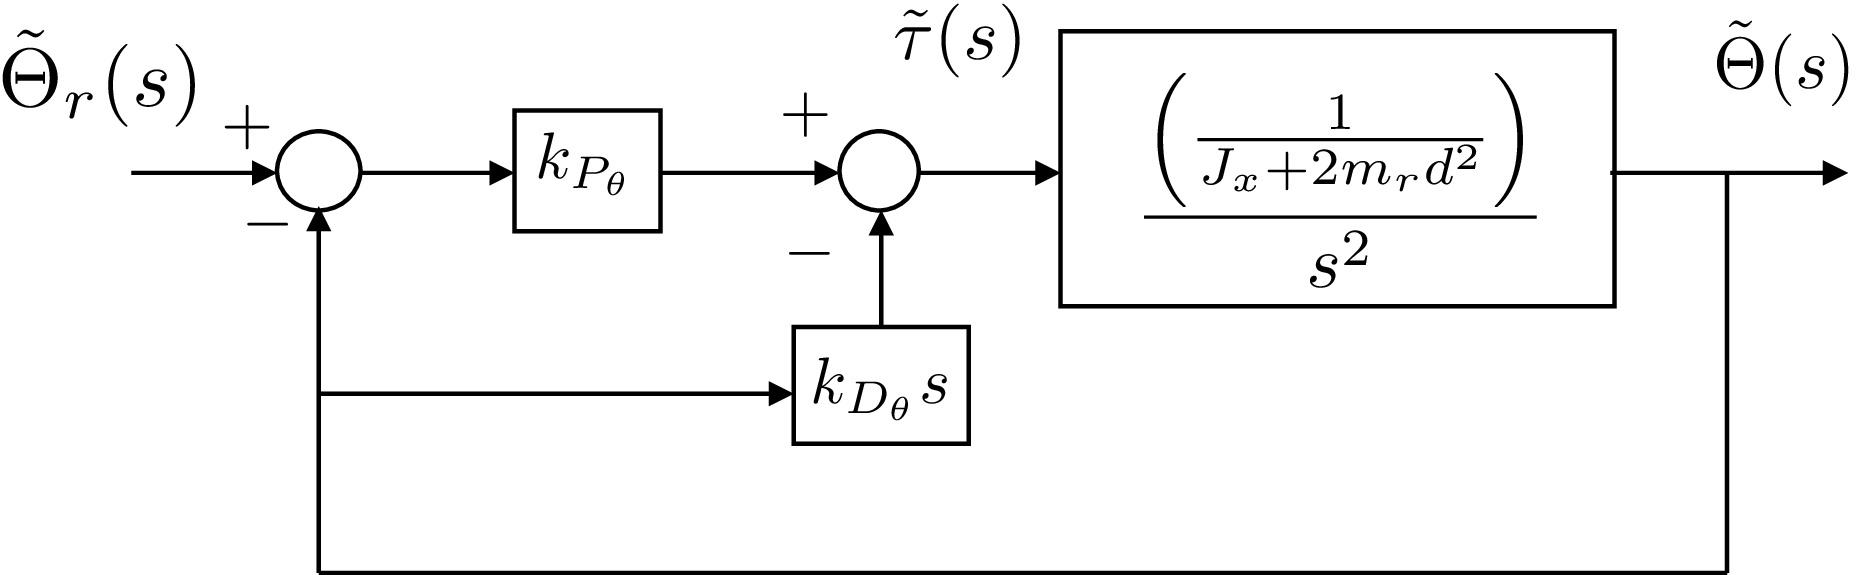
\includegraphics[width=0.8\textwidth]{6_design_studies/figures/hw_vtol_PD_inner.pdf}
   \caption{Block diagram for inner loop of the VTOL lateral controller.}
   \label{fig:hw_vtol_PD_inner}
\end{figure}

The closed loop transfer function from $\tilde{\Theta}_r$ to $\tilde{\Theta}$ is given by
\[
\tilde{\Theta}(s) = \frac{\frac{k_{P_\theta}}{J_c+2m_rd^2}}{s^2+\frac{k_{D_\theta}}{J_c+2m_rd^2}s+\frac{k_{P_\theta}}{J_c+2m_rd^2}} \tilde{\Theta_r}(s).
\]
Therefore the closed loop characteristic equation is
\[
\Delta_{cl}(s) = s^2+\frac{k_{D_\theta}}{J_c+2m_rd^2}s+\frac{k_{P_\theta}}{J_c+2m_rd^2}.
\]
The desired closed loop characteristic equation is
\[
\Delta_{cl}^d(s) = s^2 + 2\zeta_{\theta}\omega_{n_\theta} s + \omega_{n_\theta}^2,
\]
where
\begin{align*}
t_{r_\theta} &= 0.8 \\
\omega_{n_\theta} &= \frac{2.2}{t_{r_\theta}} = 2.75 \\
\zeta_{\theta} &= 0.707.
\end{align*}
Therefore
\begin{align*}
k_{P_\theta} &= w_{n_\theta}^2(J_c+2m_rd^2) = 0.3721 \\
k_{D_\theta} &= \zeta_{\theta}\omega_{n_\theta}(J_c+2m_rd^2) = 0.1913.
\end{align*}
The DC gain of the inner loop is given by
\[
k_{DC_{\theta}} = 1.
\]

Replacing the inner loop by its DC gain, the block diagram for the outer loop is shown in Figure~\ref{fig:hw_vtol_PD_outer}.
\begin{figure}[H]
   \centering
   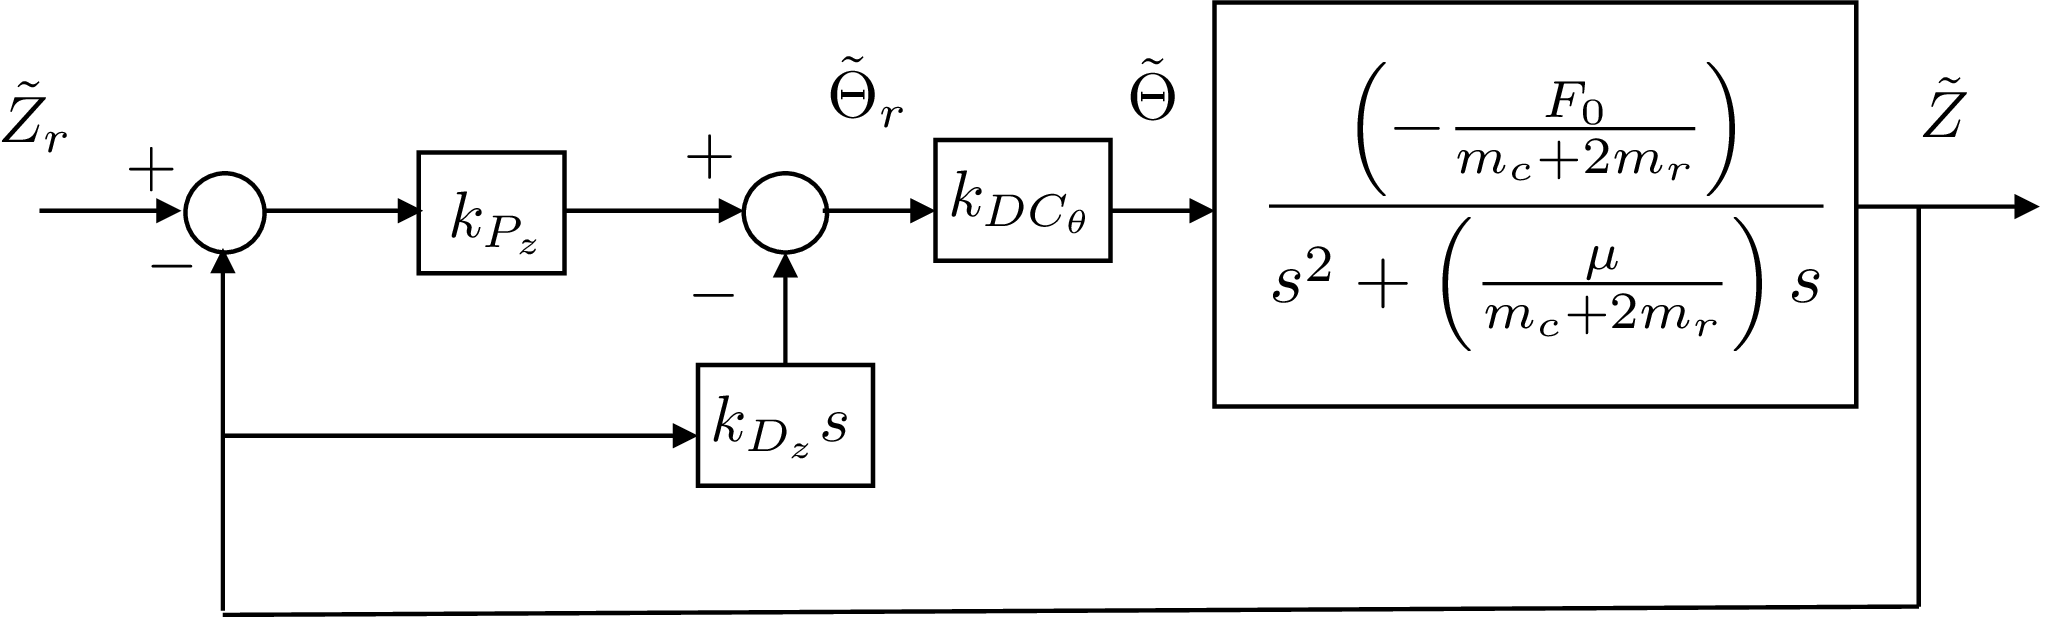
\includegraphics[width=0.8\textwidth]{6_design_studies/figures/hw_vtol_PD_outer.pdf}
   \caption{Block diagram for outer loop of VTOL lateral controller.}
   \label{fig:hw_vtol_PD_outer}
\end{figure}
The closed loop transfer function from $z_r$ to $z$ is given by
\[
Z(s) = \frac{b_1k_{P_z}}{s^2+(a_1+b_1k_{D_z})s+b_1k_{P_z}}Z_r(s),
\]
where
\begin{align*}
a_1 &= \frac{\mu}{m_c+2m_r} \\
b_1 &= \frac{-F_e}{m_c+2m_r}.
\end{align*}
The closed loop characteristic equation is therefore
\[
\Delta_{cl}(s) = s^2+(a_1+b_1k_{D_z})s+b_1k_{P_z}.
\]
The desired characteristic equation is 
\[
\Delta_{cl}^d(s) = s^2 + 2\zeta_z\omega_{n_z}s + \omega_{n_z}^2,
\]
where
\begin{align*}
t_{r_z} &= 10 t_{r_\theta} = 8 \\
\omega_{n_z} &= \frac{2.2}{t_{r_z}} = 0.2750 \\
\zeta_z &= 0.707.
\end{align*}
The PD gains are therefore
\begin{align*}
k_{P_z} &= -\frac{\omega_{n_z}^2}{b_1} = -0.0077 \\
k_{D_z} &= -\frac{2\zeta_z\omega_{n_z}-a_1}{b_1} = -0.0328.
\end{align*}


The Python, Matlab, and Simulink file associated with this problem is included on the wiki associated with the book.
    